\begin{sadlist}[h]{\ucsproblem[c]}{Decription of the use case submit problem.}{fig:ucsproblem}
\sadb{Use Case:} \ucsproblem[c] is initialized when a \aclient{} has a problem and wishes to submit that problem to the system in order to get help from the \astaff{}. 
He first has to select a category and from that choose one or more tags, he can change category and select even more tags. 
When the \aclient{} is done selecting tags the system compares the selected tags with other problems. 
If similar problems is found the \aclient{} is presented for the problems.
if one of these matches his particular problem, he can subscribe to the problem(if not closed), reopen problem(if closed), or use the information in the old problem to solve his problem independently. 
If no similar problem were found the \aclient{} creates a problem with a description and the previously selected tags. 
\sadb{Objects:} Problem, solution, tag, category, \client. (Department)

\sadb{Functions:} Search existing problems, compare problems, create problem, attach user to problem.


\end{sadlist}

\begin{figure}[htbp]
\begin{center}
 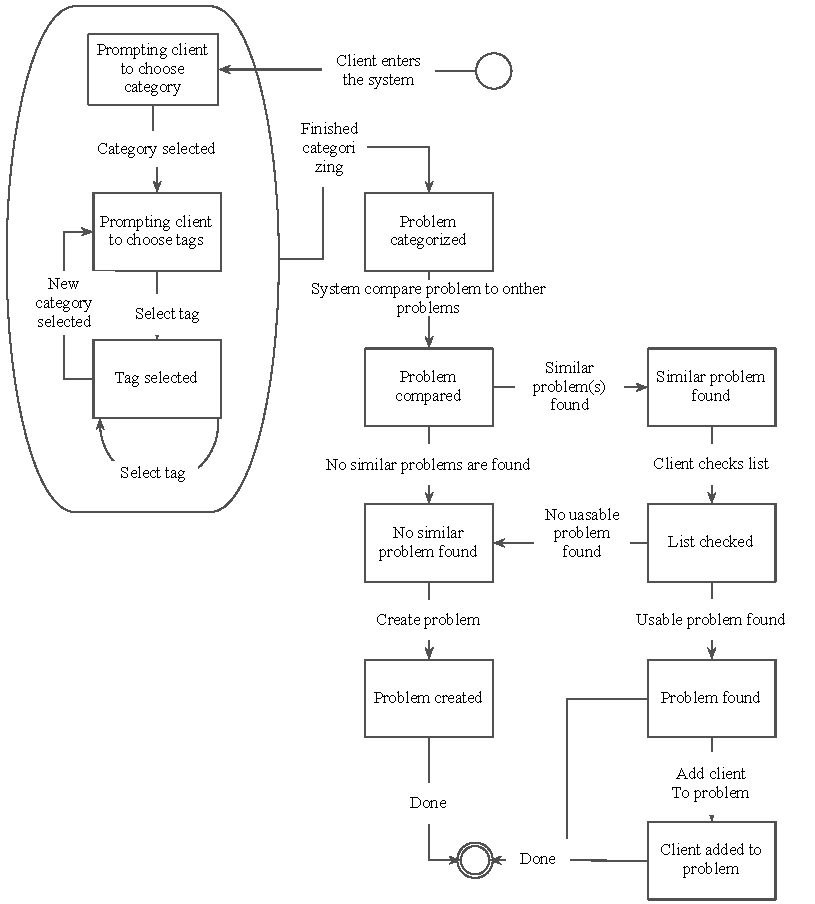
\includegraphics[scale=1]{input/application_domain_analysis/submit_problem_use_case}
\caption{default}
\label{default}
\end{center}
\end{figure}
